\section{Rupture: An improved attack}\label{subsec:rupture}
Our contributions include the development of a production-grade
framework for implementing this class of attacks called Rupture.
Rupture was developed as part of the work on extending the BREACH attack against
modern systems and block ciphers.

Rupture offers the ability to inject malicious code in any computer in the
network. This code issues requests to the endpoint and serves as a caller of
the reflection oracle that is the endpoint.

Furthermore, it enables the traffic inspection and analysis of packet
lengths. Encrypted network packets serve as the response $c_i$ from the
reflection oracle and the length of each packet is visible on the network and
captured.

In addition, Rupture offers multiple instances of the oracle $\mathcal{O}_R$, based
on various $Q$ described in \ref{subsec:parallel}, and enables the automated
computation of the reflection strings in each stage of the attack.

Finally, it amplifies the attack by issuing multiple requests per candidate
symbol in the alphabet $\Sigma$ in order to demonstrate better probability of
success. This is achieved by grouping requests in samplesets, where each
sampleset contains requests on a symbol in the alphabet $\Sigma$. Requests in a
sampleset may be constructed to enable optimization methods described in
\ref{subsec:blockalign} and \ref{subsec:parallel}.

The encrypted data pertaining to one response is a \textit{sample}.  The set of
samples collected for a particular work are a \textit{sampleset}. A work
represents the set of requests needed per candidate in the secret's alphabet.

The attack is conducted in \textit{rounds}. In each round, a decision is made
about the state of the attack and more becomes known about the secret. In a
round, either the next byte of the secret becomes known, or the known alphabet
is drilled down to a smaller set. In order to compare various different
candidate alphabets, the attack executes a series of \textit{batches} of data
collection for each round.

In each batch, several works are issued and samples are collected from each probability distribution
pertaining to a candidate alphabet, forming a sampleset. When samplesets of the
same amount of samples have been collected for all the candidate alphabets,
a batch is complete and the data is analyzed. The analysis compares the samples
of different candidates and decides which is optimal, i.e. which candidate is
contains the correct guess. This decision is made with some \textit{confidence},
is expressed in bytes. If the confidence is insufficient, an additional
batch of samplesets is collected, and the analysis is redone until the
confidence value surpases a given threshold.

Once enough batches have been collected for a decision to be made with good
confidence, the round of the attack is complete and more information about the
secret becomes known.

\subsection{Block alignment}\label{subsec:blockalign}
Block ciphers are \textit{length monotonic}, but not \textit{strictly length
monotonic}, as described in section \ref{subsec:lenmonotone}. Specifically, the
length of the encrypted text is rounded up to a product of $\mu$-bits, where $\mu$
is the block size, using added padding. The same applies for stream ciphers,
whose functionality is similar to block ciphers with block size 1 byte. In this
case, plaintext length difference between two messages does not always result in
length difference between the respective encrypted ciphertext.

It is possible to bypass this problem by using block alignment. Block alignment
techniques have already been explored in the literature \cite{moller2014poodle}. This method
demands issuing multiple requests to the reflection oracle while including
artificial noise in the reflection string $r$.

In each request $r_{i, c}$ for each candidate $c$ in the secret alphabet, we add
increasing artificial noise. That way, all $r_{1, c}$ for all c in candidates
will contain one character of alignment noise, $r_{2, c}$ will contain two
characters and so forth. As mentioned above, the difference in length of the
compressed plaintext for the correct candidate and an incorrect one is 1 byte.
For some alignment noise length $a \in [0, \mu)$ the reflection of the correct
candidate will be $(\delta*\mu)$ and for all incorrect candidates
$(\delta*\mu)+1$. In that case, the incorrect candidates result in one more
block over the network compared to the correct one.  This ensures that one out
of $\ceil{\mu / |r_i|}$ requests will result in a block distinction between the
alphabet candidates.

Figure \ref{fig:block_alignment} intuitively depicts the block alignment technique.

   \begin{figure}[thpb]
      \centering
          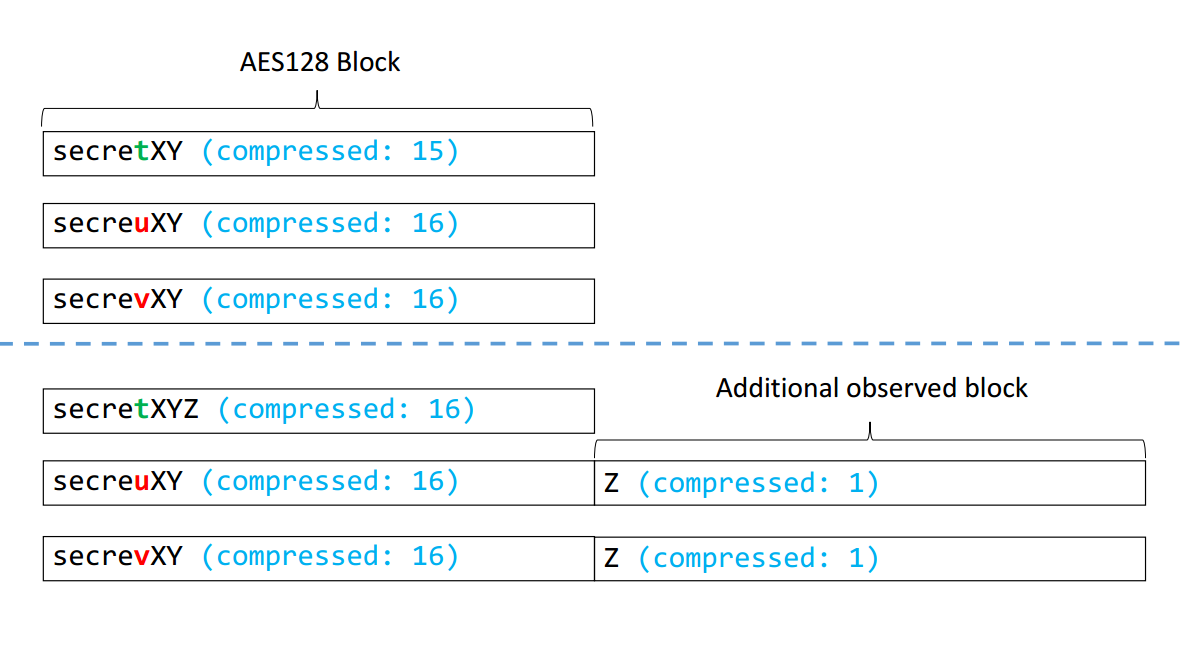
\includegraphics[width=0.48\textwidth]{figures/block_alignment.png}
      \caption{The block alignment method}
      \label{fig:block_alignment}
   \end{figure}

\subsection{Reflection computation methods}\label{subsec:reflectionmethods}
The reflection strings $r$ should be polynomially computable, as defined in
\ref{sec:propertycom}. BREACH is
parameterized with an alphabet of ASCII symbols $\Sigma$
for each character of the
secret. A successful attack should distinguish a single character of the
alphabet as the correct one through a series of requests to the reflection
oracle.

The first method of issuing requests is serial. Each request to the oracle
corresponds to a single character of the alphabet. An attack phase is completed
when requests have been issued for the entire alphabet.

In this case, $Q$ is the predicate "Given a known prefix $p_s$ of secret $s$ and
a symbol $t \in \Sigma$, is $p_s || t$ a prefix of $s$?". The complexity of the attack is $\mathcal{O}(|\Sigma|)$ and
the round ends by finding a character of the secret. This method is similar to
how BREACH previously worked.

The second method of attack is divide and conquer. In each phase the alphabet is
divided into two subsets $\Sigma_1$ and $\Sigma_2 =
\Sigma
\setminus \Sigma_1$, where $|\Sigma_1| = |\Sigma_2| =
\ceil{|\Sigma| / 2}$. The reflection string for $\Sigma_1$ consists of
$|\Sigma_1|$ substrings divided by an annotation symbol $\beta$ which is not
present in the regular plaintext. Each
substring consists of the known part of the secret concatenated with a character
in $\Sigma_1$. The reflection string for $\Sigma_2$ is constructed
similarly. For example, if $\Sigma_1$ is $\{"1", "2"\}$ and the known prefix is
"abc", using "-" as $\beta$ the reflection is: "abc1-abc2".
Each phase consists of one call to the reflection oracle per subset.

The predicate $Q$ in this case is "Given a known prefix $p_s$ of the secret $s$, is
$p_s || t$ a
prefix of $s$, where $t \in \Sigma_1$?". As long as the prefix of the
secret is \textit{compression-detectable} by each substring of the reflection,
the end of each phase marks the choice of subset $\Sigma_i$ that contains
the correct alphabet symbol and the same method is applied using chosen
$\Sigma_i$ as the alphabet $\Sigma$. The round is complete when
$|\Sigma| = 1$. Each round reduces the alphabet by half, so the complexity
of the attack with the divide and conquer method  is
$\mathcal{O}(log|\Sigma|)$.

Figure \ref{fig:divide_and_conquer} shows the reflection sequence for the case
when the alphabet is the number digits. In order to find the correct leaf of the
tree, we construct two reflections in each round. The two reflections contain
the children nodes of the parent node that was chosen in the previous round,
beginning with the root of the tree. After traversing the tree, we reach the
correct choice which is number 3.

   \begin{figure}[thpb]
      \centering
          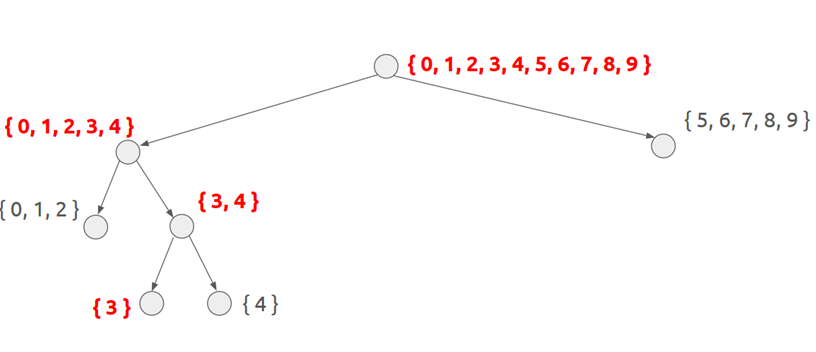
\includegraphics[width=0.48\textwidth]{figures/divide_and_conquer.png}
      \caption{The divide \& conquer method}
      \label{fig:divide_and_conquer}
   \end{figure}

\subsection{Request parallelization}\label{subsec:parallel}
The reflection oracle is generally considered synchronous. However, this is not
always the case, since it may be able to handle multiple parallel requests from
the adversary.

This is the case for the oracle in BREACH. Here the reflection oracle is an endpoint
offered by a web application and the communication channel between the adversary
and the oracle is the end-to-end browser-server network channel.

Modern web servers are able to handle multiple parallel requests and
browsers can issue a certain amount of parallel requests per domain. This
functionality enables the adversary to issue multiple parallel requests per
symbol in alphabet $\Sigma$ and efficiently reduce the execution time of
the attack.

\subsection{Request soup}
Previous sections demonstrated the need for multiple requests per reflection
string $r_i$. However, it is often the case that communication with the
reflection oracle is time
expensive. In this case, it is preferable to issue multiple
requests for a candidate and treat them as a set rather than separately.

This technique is useful in the case of BREACH. Communication between the browser and the
endpoint is encrypted, so the time needed for the analysis of
the captured packets depends on the request set.

A request set consists of requests for a symbol $s_i$ in alphabet
$\Sigma$.
Bigger request sets result in less time delay. Length calculation per request
can then be measured as the mean length over the number of requests in the set.

This method can be combined with the other methods described in this section
in order to utilize parallelization and boost the performance for
multiple requests.

\subsection{Rupture architecture}\label{app:rupture}
Rupture is a service-based architecture framework which contains multiple
independent components. While the components are designed to be able to run
independently on different networks or computer systems, easy instances of the
attack can be performed by running all subsystems on an individual system.

The framework assumes a \textit{target} service to be attacked. Typically
this target is a web service which uses TLS and
provides HTTPS endpoints. However, this assumption can
be relaxed and attacks against other similar protocols are possible. Any
protocol that exchanges encrypted data on the network and for which
the attack assumptions hold can in principle be attacked using Rupture. We
designed Rupture to be a good playground for experimentation for such new
attacks. Examples of other encrypted protocols for experimentation
include SMTP and XMPP.

The attack also assumes a user of the target service for which data will be
decrypted, the \textit{victim}. The victim is associated with a particular
target.

There are two underlying assumptions in our attack: The injection and the
sniffing assumptions. These are often, but not necessarily, achieved through the same means.

The injection assumption states that the adversary is able to inject code to the
victim's machine for execution. This code is able to issue adaptive requests to
the target service. Injection in Rupture is implemented by the
\textit{injector} component. The code that is injected is the \textit{client}
component.

The sniffing assumption states that the adversary is able to observe encrypted network
traffic between the victim and the target.
Sniffing is achieved through the \textit{sniffer}component.

The client must issue adaptive requests. For this purpose, it receives commands
through a \textit{command-and-control} channel. These commands are sent to the
client from the \textit{realtime} component with which the client maintains a
persistent connection.

The realtime component is only responsible for communicating with the client.
The actual decisions for the attack are driven by the \textit{backend}, which
maintains a persistent attack state. The backend stores persistent data in a
\textit{database} and receives data from the sniffer to perform analyses.

The various components are described in detail in the next sections.

\subsubsection{Client}

The client component is a Javascript code that issues requests towards a chosen
endpoint. This endpoint serves as the reflection oracle of the attack. The client
needs to be executed from the browser of the victim that the adversary is trying
to steal secrets from. That way, the victim's authentication cookies are
included in the request and the secrets are included in the
response.

The client contains minimal logic. It connects to the realtime service through
a command-and-control channel and registers itself. Then it waits
for work instructions by the command-and-control channel. The
client does not take any decisions or receive data about the progress of the
attack other than the work it is requested to do.
This allows the system to be upgraded without having to deploy a
new client at the victim's network.

As a regular user is browsing the Internet, multiple clients will be
injected in insecure pages and run under various contexts. All of
them register and maintain an open connection through a
with the realtime service. The realtime
service will activate one of them for this victim while keeping the others
dormant. The activated one will then receive work instructions. If the enabled
client dies, for example by closing the browser
tab, one of the rest of the clients will be woken up to continue the
attack.

\subsubsection{Injector}

The injector component is responsible for injecting the client to the victim's
browser. The injection is performed by ARP spoofing the local
network and forwarding all traffic in a Man-in-the-Middle manner. The fact that all HTTP
responses are infected increases robustness.

The injector component runs on the victim network and is
light-weight and stateless. It can be easily deployed on a small machine and
used for massive attacks. Multiple injectors can be deployed to different
networks, all controlled by the same central command-and-control channel.

\subsubsection{Realtime}

The realtime service is a service which awaits for work requests by clients. It
can handle multiple targets and victims. It receives command-and-control
connections from various clients which may live on different networks,
orchestrates them, and tells them which ones will remain dormant and which ones
will receive work, enabling one client per victim.

It maintains open web socket connections with clients and
connects to the backend service, facilitating the communication between the two
ends.

\subsubsection{Sniffer}

The sniffer component is responsible for collecting data from the
victim's network. As the client issues the requests, the sniffer
collects the ciphertext of the requests and responses as they
travel on the network. This encrypted data is then transmitted to the backend
for further analysis and decryption.

The sniffer exposes an HTTP API which is utilized by the backend for controlling
when sniffing starts, when it is completed, and retrieving the sniffed data.

\subsubsection{Backend}

The backend component is a Python code that controls the attack execution. It
initializes the attack and calculates the request sets that should be
collected. It is responsible for strategic decision taking, statistical
analysis of collected samples, adaptively advancing the attack, and storing
persistent data about the attacks in progress for future analysis.

It communicates with the realtime component in order to guide the client as to
what requests need to be made at each stage of the attack. Meanwhile, it orders
the sniffer to listen and report network traffic, which stored
at the end of each phase of the attack. The backend analyzes the
network data and calculates the confidence in the success for the attack. At the
end of each round, the predicate $Q$ is detected, depending on which method of
the ones described
in \ref{subsec:reflectionmethods} is used.

   \begin{figure}[thpb]
      \centering
          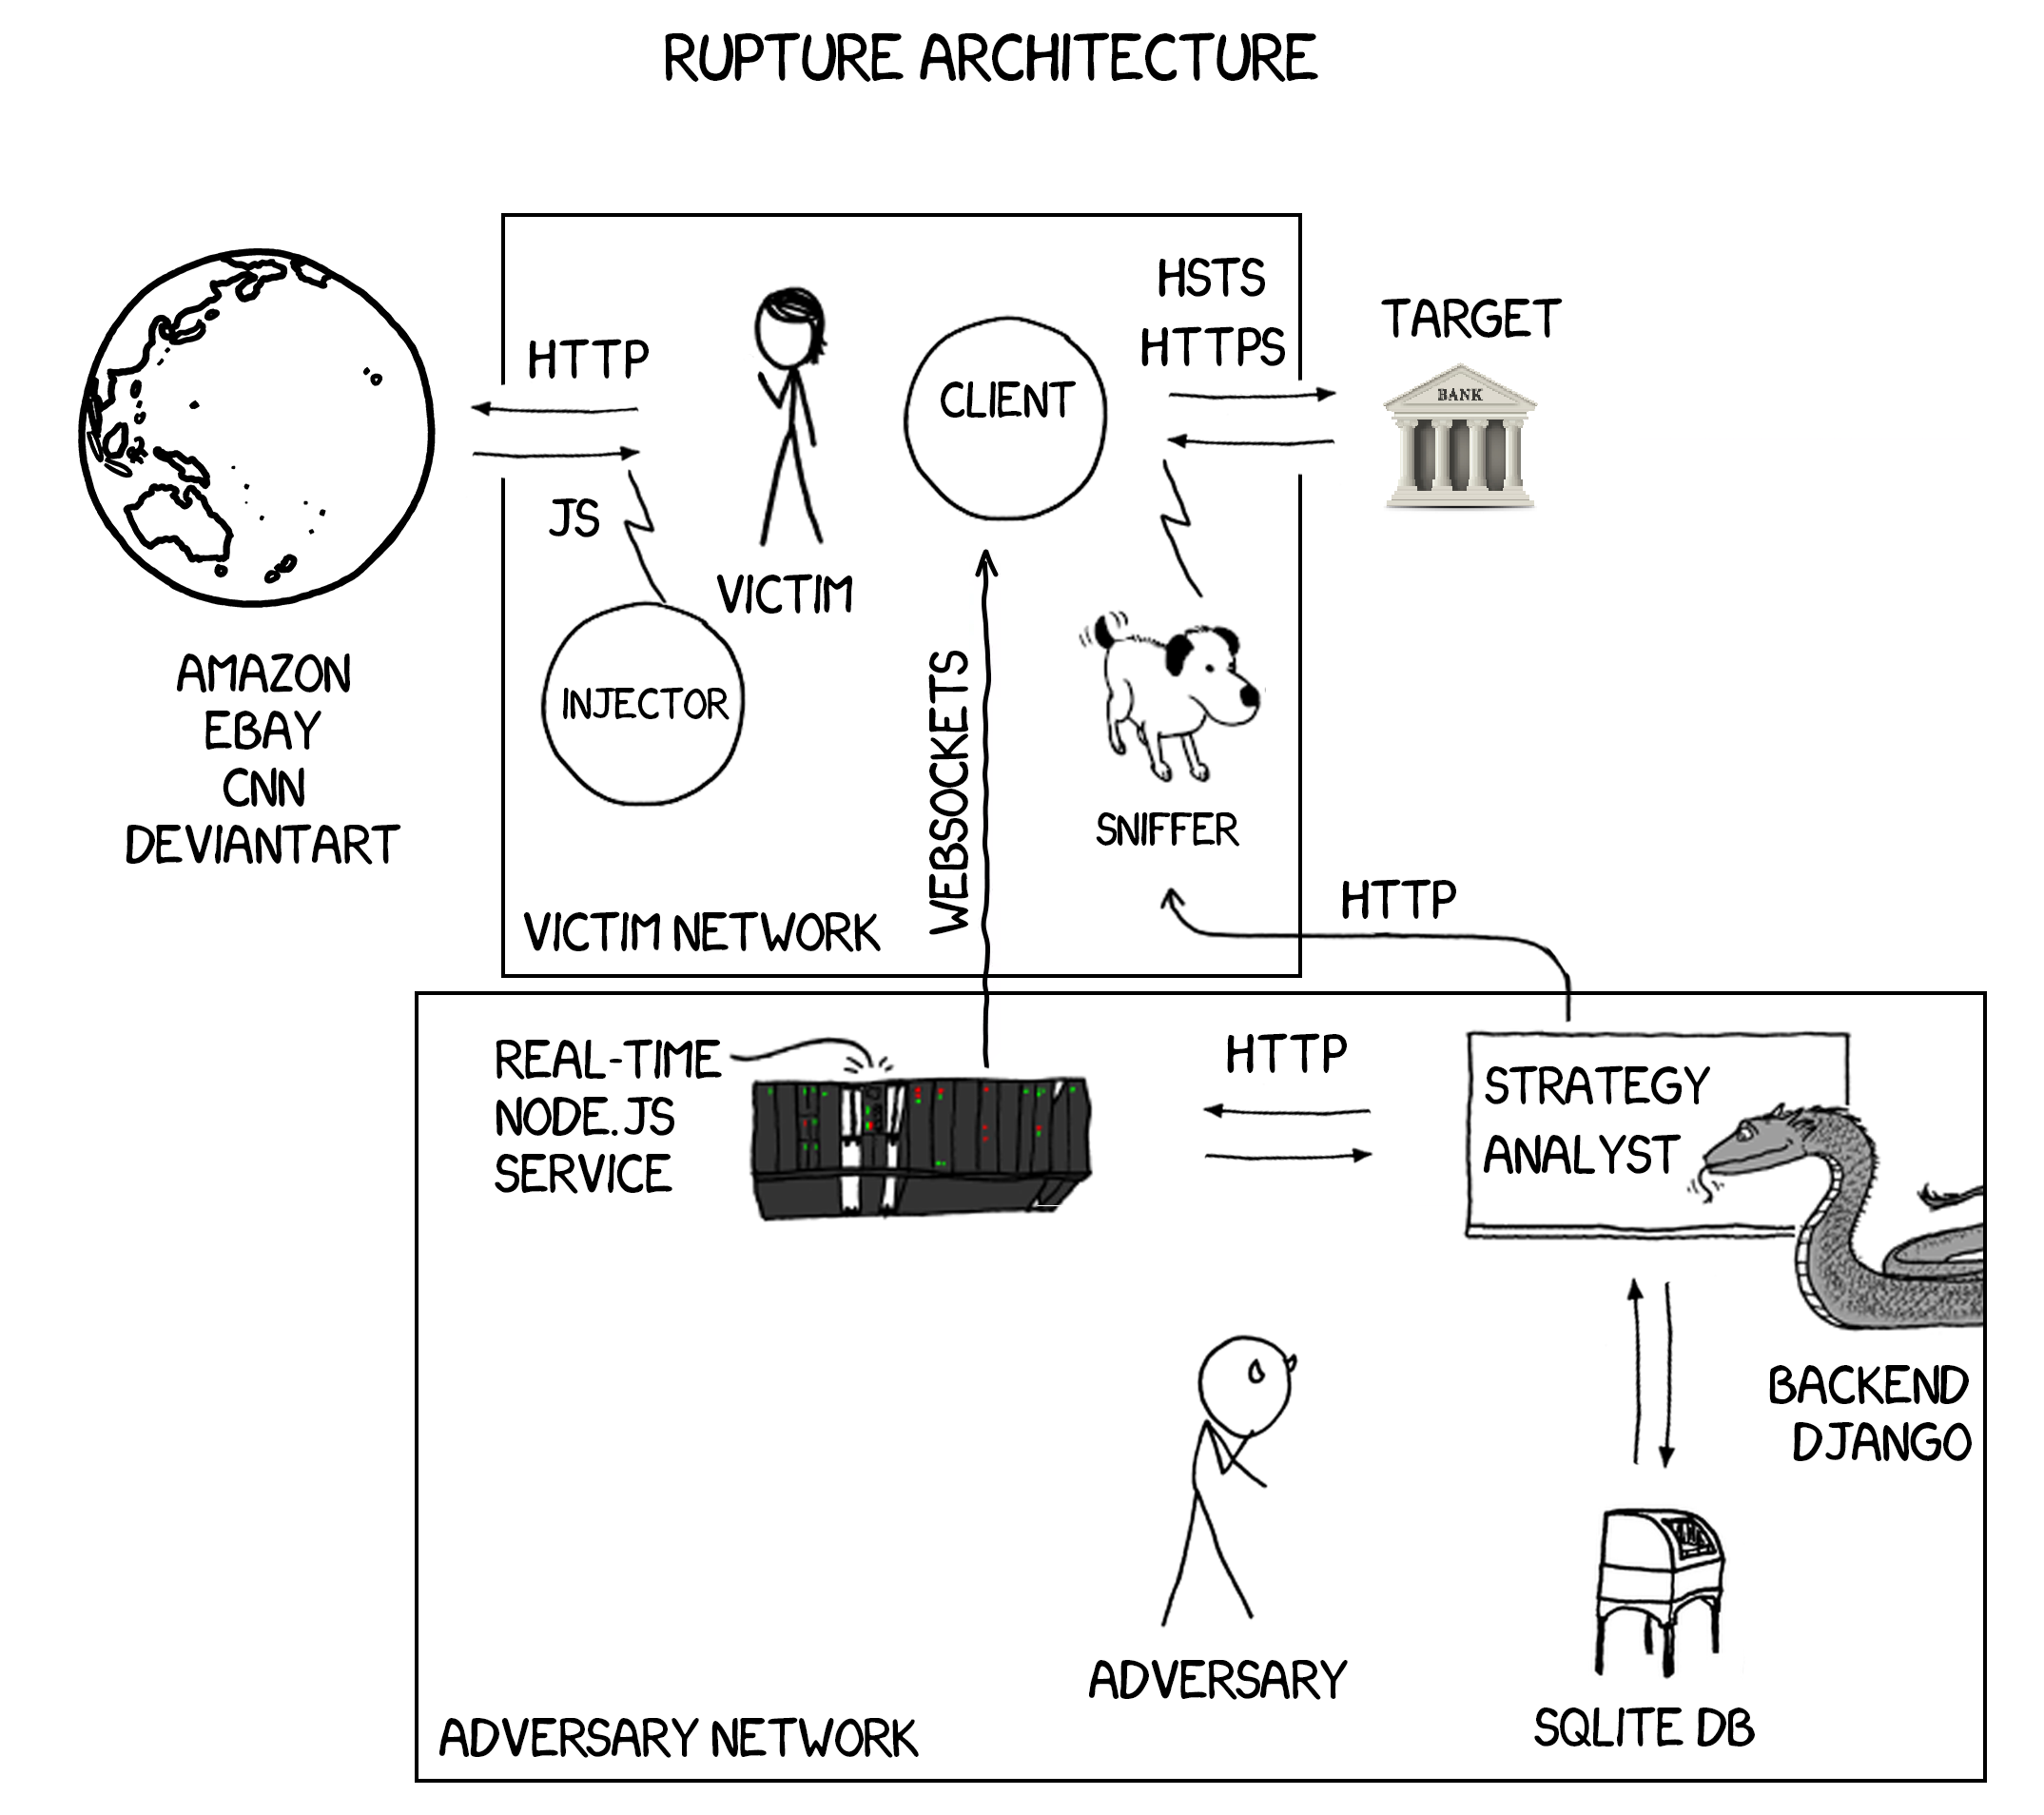
\includegraphics[width=0.48\textwidth]{figures/architecture.png}
      \caption{Rupture Architecture}
   \end{figure}
